\documentclass[slidestop,compress,mathserif,color,12pt]{beamer}

\usepackage[utf8]{inputenc}
%\usepackage[french]{babel}
\usepackage[T1]{fontenc}
\usepackage{listings}
\usepackage{multirow}
\usepackage{colortbl}


%\usetheme{Frankfurt} % Beamer theme v 3.0
\usetheme{Boadilla}
\definecolor{lightBlue}{cmyk}{0.3,0.15,0.05,0}
\definecolor{OliveGreen}{cmyk}{0.64,0,0.95,0.40}
\lstset{basicstyle=\small,backgroundcolor=\color{lightBlue},stringstyle=\ttfamily,keywordstyle=\ttfamily\color{OliveGreen},showstringspaces=false}
\usefonttheme[onlysmall]{structurebold}
\setbeamertemplate{navigation symbols}[only frame symbol]

\usepackage[absolute,overlay]{textpos}
\usepackage{url}
\usepackage{ulem}
\usepackage{mathrsfs}
\usepackage{fancybox}
\usepackage{amsmath}
\usepackage{multirow}
\usepackage{amssymb}
\usepackage{rotating}
\usepackage{amsfonts}
%\usepackage{amsthm}
\usepackage[authoryear,round]{natbib}
\def\newblock{}
\RequirePackage{bm}
\usepackage{nicefrac}
% \usepackage{algorithm} PLEASE, USE algorithm2e. It's much nicer!
% \usepackage{algorithmic}
\usepackage[ruled,vlined,linesnumbered]{algorithm2e}
\usepackage{scalefnt}
%\input{notations.tex}

\setbeamertemplate{footline}[frame number]
\usepackage{multirow}
\graphicspath{{./images/}{./}}

%\newcommand{\argmax}{\operatornamewithlimits{argmax}}

\newcommand*{\ballref}[1]{%
    \begin{pgfpicture}{-1ex}{-0.65ex}{1ex}{1ex}
    \usebeamercolor[fg]{item projected}
    {\pgftransformscale{1.75}\pgftext{\normalsize\pgfuseshading{bigsphere}}}
    {\pgftransformshift{\pgfpoint{0pt}{0.5pt}}
      \pgftext{\usebeamerfont*{item projected}#1}}
  \end{pgfpicture}}%


\title{Exorcising the Ghost in the Machine\\
\scriptsize Synthetic Spectral Data Cubes for Assessing Big Data Algorithms}

\author{\textbf{Mauricio Araya}, Mauricio Solar, \\Diego Mardones and
Teodoro Hochf\"arber}

\date{Laboratory of Interdisciplinary Research in Astroengineering\\ Universidad Técnica Federico Santa
María\\ Chile}

\begin{document}

\begin{frame}
  \titlepage
\end{frame}

\begin{frame}
  \frametitle{Astronomical Big Data Analysis}
\Large
\pause
\centering{Machine Learning is the solution,}

\pause

\centering{right?}

\pause

\centering{No free lunch!}
\normalsize 
\begin{itemize}
\item data consuming, or...
\item highly dependent of prior knowledge
\item verifiable (labelled) real data is scarce
\item more advanced $\sim$ more complex
\item more flexible $\sim$ more parameters
\item data analysis science (study)
\item parameter tunning is a nightmare 
\end{itemize}
\pause

\huge
\centering{We need synthetic data!}
\end{frame}

\begin{frame}
  \frametitle{Astronomical SYnthetic Data Observations \\(ASYDO)}
\begin{itemize}
\item \textbf{Synthetic} ALMA-like data generator
\item \textbf{Simple/mock} astrophysical models
\item \textbf{Arbitrary} data cubes observations (FITS)
\item Opportunity for Machine Learning
\begin{itemize}
   \item Labelled and reliable data
   \item Unbounded number of samples
   \item Data-driven sensitivity analysis
\end{itemize}
\item Opportunity for information technologies in general
\begin{itemize}
   \item Assessment of bulk-data transfer, compression, etc.
   \item Assessment of image analysis techniques
   \item Assessment of storage systems
\end{itemize}
\end{itemize}
\end{frame}

\begin{frame}
  \frametitle{Data Cube Characterization}
\scriptsize
\begin{minipage}{0.65\linewidth}
A spectroscopic data cube with calibrated temperatures,
with two spatial axes 
and a frequency axis.

Basic model:
\begin{equation}
C(x,y,f) = \hat{C}(x,y,f) + \mathcal{N}(0,\sigma)
\end{equation}

What to simulate in $\hat{C}(x,y,f)$?
\begin{itemize}
\item Emission lines frequency, energy, etc (DB)
\item Local radial velocity gradients
\item Red-shift correction
\item Broadening functions (frequency distribution model)
\item Reasonable spatial distribution models
\end{itemize}



\end{minipage}
\hfill
\begin{minipage}{0.29\linewidth}
\includegraphics[width=0.99\linewidth]{spectralcube.jpg}
\vskip1cm
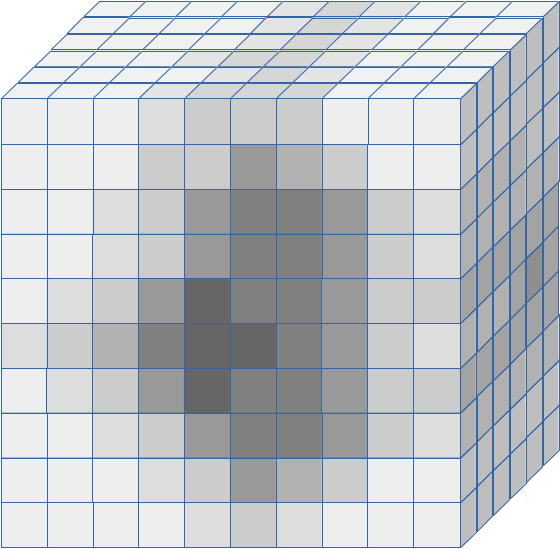
\includegraphics[width=0.99\linewidth]{cube.png}\\
\end{minipage}
\end{frame}


%\begin{frame}
%  \frametitle{Spectral Lines}
%\begin{itemize}
%\item Gaussiana
%\end{itemize}
%\includegraphics[width=0.3\linewidth]{images/splata.jpg}
%\hfill
%\includegraphics[width=0.3\linewidth]{images/spectralcube.jpg}
%\hfill
%\includegraphics[width=0.3\linewidth]{images/lines2.png}
%\end{frame}


\begin{frame}
  \frametitle{Data Cell Characterization}
\scriptsize
\only<1>{\centerline{\includegraphics[width=0.65\linewidth]{line-block.png}}}
\only<2>{\centerline{\includegraphics[width=0.25\linewidth]{line-block.png}}}

The temperature of a cell is given by the following model:
\begin{equation}
C(x,y,f)=\sum_{l \in \mathcal{L}(x,y,f,l)}
\int_{\nu_f - \Delta
\nu/2}^{\nu_f + \Delta \nu/2} 
Br(\nu,l)df + \epsilon
\label{eq:base}
\end{equation}

\begin{example}
By assuming a Gaussian line profile,
\begin{equation}
C(x,y,f)=\sum_{l \in \mathcal{L}(x,y,f,l)}
\int_{\nu_f - \Delta
\nu/2}^{\nu_f + \Delta \nu/2} 
\frac{T_l(x,y)}{S_l(x,y) \sqrt{2\pi}}exp\left(- \frac{(\nu - \nu_l(1 +
Z_l(x,y)))^2}{2S_l(x,y)^2}\right) df +
\epsilon
\label{eq:base}
\end{equation}
\end{example}

For each line $l$ we need to generate $T_l$ (temperature),
$Z_l$ (redshift) and broadening parameters $\Phi_l$ 
(i.e. $S$ in example)
\end{frame}


\begin{frame}
  \frametitle{ASYDO Elements}
\scriptsize
\begin{minipage}{0.39\linewidth}
\only<1>{
\centerline{\includegraphics[width=0.97\linewidth]{internal.png}}

\centerline{\includegraphics[width=0.7\linewidth]{comp.png}}}
\only<2>{\centerline{\includegraphics[width=0.97\linewidth]{archi.png}}

\centerline{\includegraphics[width=0.97\linewidth]{comp_all.png}}}
\end{minipage}
\begin{minipage}{0.59\linewidth} 
Elements:
\begin{itemize}
\item Persistent object called Virtual Universe (VU)
\item Sources that belongs to VU ($\alpha_S$,$\delta_S$,$z_S$).
\item Sources have several components (structures)
\item Components use a models 
      \begin{itemize}
     \item \scriptsize Molecular Clouds, PDR, blackbody, continuum
		\end{itemize}
\item A model generates each $T_l$, $Z_l$ and $\phi_l$ 
\item Arbitrary observations
      \begin{itemize}
     \item \scriptsize Angular position ($\alpha$,$\delta$)
     \item Angular resolution $\Delta\theta$ and the Field of View (FOV)
     \item Central frequency $\nu$, spectral resolution ($\delta \nu$) 
		and spectral bandwidth (BW)
   \end{itemize}
\end{itemize}
Modules:
\begin{itemize}
\item \texttt{asydopy.vu} virtual universe (asydo core)
\item \texttt{asydopy.db} line database manipulation (SLAP service)
\item \texttt{asydopy.factory} generate randomized cubes
\end{itemize}
\end{minipage}
\end{frame}


\begin{frame}
  \frametitle{Tools for the Models}
\scriptsize
\begin{minipage}{0.63\linewidth} 
\begin{itemize}
\item Spatial structures
   \begin{itemize}
      \item \scriptsize Gaussian 2D
      \item Generalized Gaussian 2D (saturated, Lorenzian, etc)
      \item Exponential
      \item Soft-edge rings (TODO)
      \item Random Clouds (TODO)
   \end{itemize}
\item Spectral form
   \begin{itemize}
     \item \scriptsize Skew-Normal Distribution (1D)
   \end{itemize}
\item Local shift functions
   \begin{itemize}
     \item \scriptsize Linear
     \item Exponantial
   \end{itemize}
\end{itemize}
\end{minipage}
\begin{minipage}{0.33\linewidth}
\includegraphics[width=0.8\linewidth]{gauss.jpg}\\
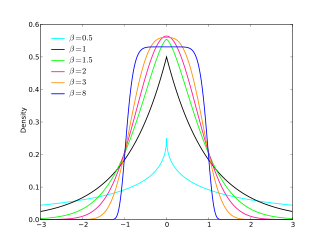
\includegraphics[width=0.49\linewidth]{gg.png}
\includegraphics[width=0.49\linewidth]{gg2.png}\\
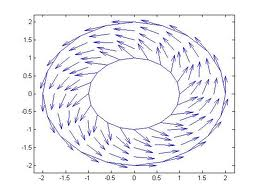
\includegraphics[width=0.8\linewidth]{ring.jpg}
\end{minipage}
\end{frame}


%\end{minipage}

%\hfill
%\begin{minipage}{0.29\linewidth}
%\begin{block}{\scriptsize Matrix Generation Example}
%\scriptsize
%$T_m(x,y) = GM(x,y;s_{maj},s_{min},\theta,\alpha,\delta)$  \\
%$Z(x,y) = z + grad(x,y,\alpha,\delta,\phi)$
%end{block}
%\end{minipage}
%\end{frame}

%\begin{frame}[fragile]
%  \frametitle{ASYDO Operations Overview}
%\scriptsize
%\begin{verbatim}
%Interface Universe:
%   Universe(log)
%   CreateSource(alpha,delta,redshift)
%   AddComponent(name,model)
%   genCube(name,cubespec,filename)
%
%Structure CubeSpec(alpha,delta,freq,ang_res,ang_fov,spe_res,spe_bw)
%
%Interface Component:
%   Component(mod_params)
%   project(cube)
%   register(comp_name,alpha,delta)
%   setRadialVelocity(rv)
%
%Interface Line:
%   Line(spe_form)
%   genLine(freq,freq_axis)
%
%Interface Surface:
%   Surface(spa_form)
%   genSurface(alpha,delta,alpha_axis,delta_axis)
%
%\end{verbatim}
%\end{frame}

\begin{frame}
  \frametitle{What we save in the FITS?}
\begin{minipage}{0.62\linewidth}
\scriptsize
\begin{itemize}
\item A 3D image (cube)
\item For each component (and subcomponent) we have
\begin{itemize}
   \item \scriptsize 2D images with the original matrices
   \begin{itemize}
      \item \scriptsize Temperature ($T_m$)
      \item Red-shift ($Z_m$)
      \item Broadening ($\Phi_m$)
   \end{itemize}
   \item A FITS table with each line of the component 
   \item This include: 
   \begin{itemize}
		\item \scriptsize unique line code
      \item molecule name
      \item chemical name
      \item rest frequency
      \item observed frequency
      \item base red-shift
      \item temperature  
   \end{itemize}
 \end{itemize}
%\item The maximum intensity of the molecule depends on a handcrafted random
%model:
%\begin{tabular}{|c|c|c|}
%\hline
%\textbf{Molecule} & 
%\textbf{Min Int.} & 
%\textbf{Max Int.} \\
%\hline
%\hline
%CO & 20 &  60\\
%\hline
%13CO & 5 & 20\\ 
%\hline
%HCO+, HC3N, CS, C18O, CH3OH, N2H & 1 &  10\\
%\hline
%Others & 0.1 &  2\\ 
%\hline
%\end{tabular}

%Modifiers:\\
%13C = 1/30, 18O = 1/60, 17O = 1/120, 34S = 1/30,\\ 33S = 1/120, 13N= 1/30, D =  1/30
\end{itemize}
\end{minipage}
\begin{minipage}{0.33\linewidth}
\includegraphics[width=0.98\linewidth]{lines.png}\\
\includegraphics[width=0.68\linewidth]{image.png}\\
\includegraphics[width=0.68\linewidth]{image2.png}
\end{minipage}
\end{frame}

\begin{frame}
  \frametitle{Examples}
\only<1>{
Supervised Learning Example:
\begin{itemize}
\item 
\scriptsize Pick a 2GHz frequency window ($\sim$ 300 GHz)
\item Select randomly (p=0.3) if a cube have a molecule
\item Force Phosphapropynylidyne existence and abscense (Binary Class)
\item 30000 cubes, 25x25x1000 size each 
\item Naive approach: Use a SVM to train and test
\item Result: 62\% (something)
\item The ML approach is insanely simple
\end{itemize}}
\only<2->{\normalsize Line Identification Example\\(wavelet-peak-detect,
levenberg-marquardt gaussian fitting)}
\only<2>{\includegraphics[width=0.93\linewidth]{good_fit.png}}
\only<3>{\includegraphics[width=0.93\linewidth]{noisy_fit.png}}
\only<4>{\includegraphics[width=0.93\linewidth]{notsogood_fit.png}}
\only<5>{\includegraphics[width=0.93\linewidth]{verynoisy_fit.png}}
\only<6>{\includegraphics[width=0.93\linewidth]{toomany_fit.png}}
\end{frame}

\begin{frame}
  \frametitle{Future Work}
\scriptsize
\begin{itemize}
\item Virtual Universe Service!
\centerline{\includegraphics[width=0.45\linewidth]{digital_universe.jpg}}
\item IVOA-like synthetic data generation standard (web)
\item Include more models and tools
\item Integration with \texttt{astropy} and/or CASA
\item Train using \textbf{synthetic data}, test using \textbf{real data}
\end{itemize}
\end{frame}

\begin{frame}
  \titlepage
\end{frame}

\begin{frame}
  \frametitle{Skew-normal Distribution}
\scriptsize
\begin{itemize}
\item The pdf of the skew normal (SN) distribution is:
\begin{equation}
f(x) = \frac{2}{\omega}\phi\left(\frac{x-\xi}{\omega}\right)\Phi\left(\alpha
\left(\frac{x-\xi}{\omega}\right)\right)
\end{equation}
where $\phi(x)=\frac{1}{\sqrt{2\pi}}e^{-\frac{x^2}{2}}$ is the standard normal
pdf and $\Phi(x) = \frac{1}{2} \left[ 1 +
\operatorname{erf} \left(\frac{x}{\sqrt{2}}\right)\right]$ the standard normal
cdf.
\item The parameters of $SN(\xi,\omega,\alpha)$ are $\xi$=location,
$\omega$=scale and $\alpha$=shape
\item We propose first to reparametrize as follows
\begin{align}
\mu & =  E[X]  = \xi + \omega\delta\sqrt{\frac{2}{\pi}}\\
\sigma^2 & = E[(X-\mu)^2] = \omega^2\left(1 - \frac{2\delta^2}{\pi}\right) \\
\delta & = \frac{\alpha}{\sqrt{1+\alpha^2}}
\end{align}
which gives the following form
\begin{equation}
SN'(\mu,\sigma,a) = SN\left(\mu - \frac{\sigma \delta}{\sqrt{1 - \frac{2\delta^2}{\pi}}}
\cdot \sqrt{\frac{2}{\pi}} , \frac{\sigma}{\sqrt{1 -
\frac{2\delta^2}{pi}}},\alpha\right)
\end{equation}
\end{itemize}
\end{frame}


\begin{frame}
  \frametitle{Example: simple model}
\scriptsize
%\begin{minipage}{0.65\linewidth}
%\scriptsize
Defining $T_l$, $Z_l$ y $\Phi_l$ matrices for each line is tedious.
Group by molecules: 
\begin{itemize}
 \item molecule intensity maps $T_m$,
 \item local molecule redshift maps $Z_m$,
 \item and molecule broadening maps $S_m$.
\end{itemize} 

\begin{minipage}{0.49\linewidth}
The molecular model need to define (simple example):
\begin{align*}
T_l & = f(T_m,l) = T_m exp\left(-\frac{|e_l - t|}{t}\right) \\
Z_l & = g(Z_m,l) = Z_m \\
\phi_l & = h(\phi_m,l) =  \frac{S_m \nu_l}{2\sqrt{2\ln 2} c}\\
T_m & = 2DGauss(\sigma_x,\sigma_y,\theta) \\
Z_m & = Linear(\alpha,\beta,\theta) \\
S_m & = s_m  \\
\end{align*}
\end{minipage}
\begin{minipage}{0.49\linewidth}
\centerline{\includegraphics[width=0.9\linewidth]{cube-thresh3.png}}
\end{minipage}
\end{frame}


\begin{frame}
  \frametitle{Spectral Line Database}
\scriptsize
\begin{minipage}{0.65\linewidth}
$\mathcal{L}$ is the set of all lines,
and $\nu_l$ the central frequency of $l \in \mathcal{L}$.
If the frequency range is constrained to
$\mathcal{R}=[\nu_{min},\nu_{max}]$, 
the set of potentials peaks in $\mathcal{R}$ is:
\begin{equation*}
\mathcal{L}_\mathcal{R} = \{ l \in \mathcal{L} | \nu_l \in \mathcal{R} \}
\end{equation*}

A line $l$ has other associated values in the DB 
such as the transition temperature $e_l$ or the molecule species $m_l$ (formula).

For example, the set of species in an arbitrary region $\mathcal{R}$ 
is defined as
\begin{equation*}
\mathcal{M}_\mathcal{R} = \{ m \in \mathcal{M} | \exists l \in
\mathcal{L}_\mathcal{R}, m=m_l \},
\end{equation*}
where $\mathcal{M}$ is the set of all the molecules in the DB.

\begin{center}
\begin{minipage}{0.90\linewidth}
\begin{block}{Assumptions}
\begin{itemize}
\item \textbf{S1}: the DB contains all the observable lines
\item \textbf{S2}: each transition has an associated molecule
\end{itemize}
\end{block}
\end{minipage}
\end{center}
\end{minipage}
\hfill
\begin{minipage}{0.29\linewidth}
\includegraphics[width=0.99\linewidth]{splata.jpg}\\
\vskip1cm
\includegraphics[width=0.99\linewidth]{molecules.png}\\
\vskip1cm
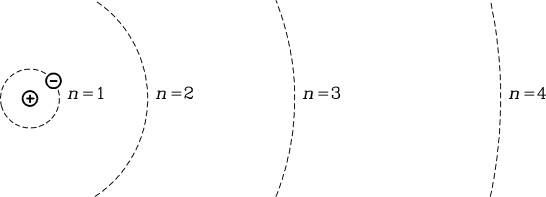
\includegraphics[width=0.99\linewidth]{recom.png}\\
\end{minipage}
\end{frame}
%
%\begin{frame}
%  \frametitle{Spectral Lines}
%\scriptsize
%\begin{minipage}{0.65\linewidth}
%
%Frequencies in DB in rest.
%Doppler effect given a reshift $z$,
%\begin{equation*}
%\nu_{obs} = \left(1 + z\right)\nu_0.
%\end{equation*}
%
%Lines have a broadening in the frequency space 
%(natural, doppler, pressure, opacity, etc).
%There are upper and lower bounds:
%\begin{equation*}
%[\nu_l^{low},\nu_l^{up}]=[low(\nu_l),up(\nu_l)].
%\end{equation*}
%
%For each line, a broadening function of $\nu$ 
%is used $Br(\nu_l,\phi_l)$:
%
%\begin{example}
%\tiny
%Using a Gaussian function:
%\begin{equation*}
%Br(\nu_l,\phi_l) = T_l Gauss(\nu_l;\sigma_l) = \frac{T_l}{\sigma_l \sqrt{2\pi}}exp\left(- \frac{(\nu -
%\nu_l)^2}{2\sigma_l^2}\right)
%\end{equation*}
%where $T_l$ is the integrated intensity of the whole line,
%and $\phi_l= \{T_l,\sigma_l\}$.
%
%Moreover, the $\sigma_l$ 
%(standard deviation) can be derived from parameters 
%such as the Full-Width at Half Maximum (FHWM):
%\begin{equation*}
%\sigma_l = \frac{fwhm_\nu}{2\sqrt{2\ln 2}} = \frac{fwhm_{rv} \cdot
%\nu_l}{2\sqrt{2\ln 2}  c}
%\end{equation*}
%\end{example}
%
%\end{minipage}
%\hfill
%\begin{minipage}{0.29\linewidth}
%\begin{center}
%\begin{minipage}{0.90\linewidth}
%\begin{block}{Assumptions}
%\begin{itemize}
%\item \textbf{S3}: $low(\cdot)$ and $up(\cdot)$ exist
%\item\textbf{S4}: $\phi_l$ is a sufficient statistic of the broadening
%\end{itemize}
%\end{block}
%\end{minipage}
%\vskip0.5cm
%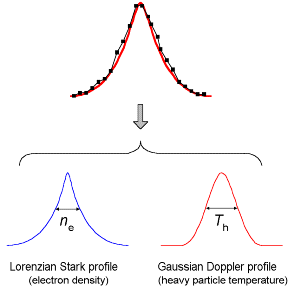
\includegraphics[width=0.99\linewidth]{lineprof.png}\\
%\end{center}
%\end{minipage}
%\end{frame}
%
\end{document}

